\documentclass[12pt,a4paper,oneside]{book} 

%%%%%%%%%%%%%%%%%%%%%%%%%%%%%%%%%%%%%%%%%%%%%%%%%%%%%%%%%%%%%%%%%%%%%%%%

\usepackage{ifthen}
\usepackage{graphicx}
\usepackage[dvips]{epsfig}
\usepackage{grffile} %Allows the graphics files to have spaces in their addresses
\usepackage{enumerate}
\usepackage{calc}
\usepackage{multicol} 
\usepackage{titlesec}
%\usepackage{showkeys}

%%%%%%%%%%%%%%%%%%%%%%%%%%%%%%%%%%%%%%%%%%%%%%%%%%%%%%%%%%%%%%%%%%%%%%%%

\usepackage{a4}
\usepackage{amsfonts}
\usepackage{amssymb}

%%%%%%%%%%%%%%%%%%%%%%%%%%%%%%%%%%%%%%%%%%%%%%%%%%%%%%%%%%%%%%%%%%%%%%%%

\usepackage{t1enc,times}
\usepackage{latexsym,amssymb}
\usepackage{amsmath}
\usepackage{amstext}
%\usepackage[T1]{fontenc}
%\usepackage{cmbright}
\usepackage{pifont}
\usepackage{marvosym}
%\usepackage{pslatex}
\usepackage{stmaryrd}
%\usepackage{txfonts}  

%%%%%%%%%%%%%%%%%%%%%%%%%%%%%%%%%%%%%%%%%%%%%%%%%%%%%%%%%%%%%%%%%%%%%%%%%%%%%%%

\usepackage{fancybox} 
\usepackage{fancyhdr}
\usepackage{fullpage}

%%%%%%%%%%%%%%%%%%%%%%%%%%%%%%%%%%%%%%%%%%%%%%%%%%%%%%%%%%%%%%%%%%%%%%%%%%%%%%%
\usepackage[left = 0.5in, right = 0.5in, top = 0.8in, bottom =1in]{geometry}
\usepackage[colorlinks=true, linkcolor = blue, citecolor = blue]{hyperref}%Coloured hyperlinks
\setlength{\columnsep}{0.3in} %column separation
%\usepackage{url}    
%\ExecuteOptions{dvips}
%\usepackage[pdftex,colorlinks=true]{hyperref}
%\hypersetup{backref,pdfpagemode=UseThumbs,pdfstartview=Fit,
%pdfpagelayout=SinglePage,pdfstartpage=1,colorlinks=true,menucolor=msc,
%anchorcolor=msc,pagecolor=msc,urlcolor=rfr,breaklinks=true,hyperfootnotes=true}

%%%%%%%%%%%%%%%%%%%%%%%%%%%%%%%%%%%%%%%%%%%%%%%%%%%%%%%%%%%%%%%%%%%%%%%%%%%%%%%

\graphicspath{{../figs/}}
\pagestyle{fancy}
\fancyhf{} 
%\renewcommand{\headrulewidth}{1pt}
%\renewcommand{\footrulewidth}{1pt}
\renewcommand{\headwidth}{\textwidth}
\fancyhead[LE]{\leftmark}
\fancyhead[RO]{\small \rightmark}
\fancyfoot[C]{\thepage}

%%%%%%%%%%%%%%%%%%%%%%%%%%%%%%%%%%%%%%%%%%%%%%%%%%%%%%%%%%%%%%%%%%%%%%%%%%%%%%%

\tolerance 4000
\textwidth 17.00cm
\topmargin -0.30cm
\oddsidemargin -0.25cm
\evensidemargin -0.25cm
\textheight 23.00cm
%\headsep 12pt
\headheight 15pt
\footskip 60pt
%\parindent 12pt

%%%%%%%%%%%%%%%%%%%%%%%%%%%%%%%%%%%%%%%%%%%%%%%%%%%%%%%%%%%%%%%%%%%%%%%%%%%%%%%

\renewcommand{\rmdefault}{ptm}  % times
\renewcommand{\rmdefault}{phv}  % helvetica
\renewcommand{\rmdefault}{pbk}  % bookman
\renewcommand{\rmdefault}{ppl}  % palatino
\renewcommand{\sfdefault}{phv}  % helvetica as sans serif
\renewcommand{\ttdefault}{pcr}  % courier as fixed width
\renewcommand{\tabcolsep}{8pt}
\renewcommand{\arraystretch}{1.25}

%%%%%%%%%%%%%%%%%%%%%%%%%%%%%%%%%%%%%%%%%%%%%%%%%%%%%%%%%%%%%%%%%%%%%%%%%%%%%%%

\def\nn{\nonumber}
\def\f{{\frac}}
\def\pa{{\partial}}
\def\d{{\rm d}}
\def\l{\left}
\def\r{\right}
\def\Mpl{M_{_{\rm Pl}}}
\def\mb{\mathbf}
\newcommand{\del}{\mathbf{\nabla}}
%%%%%%%%%%%%%%%%%%%%%%%%%%%%%%%%%%%%%%%%%%%%%%%%%%%%%%%%%%%%%%%%%%%%%%%%%%%%%%%

\def\done{\marginpar {\scriptsize DONE}}
\def\check{\marginpar {\scriptsize CHECK}}

%%%%%%%%%%%%%%%%%%%%%%%%%%%%%%%%%%%%%%%%%%%%%%%%%%%%%%%%%%%%%%%%%%%%%%%%%%%%%%%

\begin{document}

%%%%%%%%%%%%%%%%%%%%%%%%%%%%%%%%%%%%%%%%%%%%%%%%%%%%%%%%%%%%%%%%%%%%%%%%%%%%%%%

\baselineskip 20pt

%%%%%%%%%%%%%%%%%%%%%%%%%%%%%%%%%%%%%%%%%%%%%%%%%%%%%%%%%%%%%%%%%%%%%%%%%%%%%%%

\pagenumbering{roman}

%%%%%%%%%%%%%%%%%%%%%%%%%%%%%%%%%%%%%%%%%%%%%%%%%%%%%%%%%%%%%%%%%%%%%%%%%%%%%%%

\thispagestyle{empty}
\topskip 15pt
\hrule\hrule\hrule\hrule\hrule
\vskip 20pt
\centerline{\Huge \bf Mg II absorber clustering} 
\vskip 15pt
\centerline{\Huge \bf along QSO sightlines} 
\vskip 20pt
\hrule\hrule\hrule\hrule\hrule
\vskip 30pt
\centerline{\Large A project report}
\vskip 8pt
\centerline{\Large submitted in partial fulfillment 
for the award of the degree of}
\vskip 8pt
\centerline{\Large Master of Science}
\vskip 8pt
\centerline{\Large in}
\vskip 8pt 
\centerline{\Large Physics}
\vskip 8pt
\centerline{\Large by}
\vskip 8pt
\centerline{\Large \bf H S Sunil Simha}
\vskip 8pt
\centerline{\Large under the guidance of}
\vskip 8pt
\centerline{\Large  Dr. L. Sriramkumar, IIT Madras}

\vskip 8pt
\centerline{\Large  Dr. R Srianand, IUCAA, Pune}
\vskip 30pt 
\begin{center}
\epsfig{file=iitm.ps, width=3.0cm, height=3.0cm}
\end{center}
\vskip 8pt 
\centerline{\Large \bf Department of Physics}
\vskip 8pt 
\centerline{\Large \bf Indian Institute of Technology Madras}
\vskip 8pt 
\centerline{\Large \bf Chennai~600036, India}
\vskip 8pt
\centerline{\Large \bf April 2018}
%%%%%%%%%%%%%%%%%%%%%%%%%%%%%%%%%%%%%%%%%%%%%%%%%%%%%%%%%%%%%%%%%%%%%%%%%%%%%%%

\newpage\topskip 40pt
\centerline{\Large CERTIFICATE}
\thispagestyle{empty}
\vskip 20pt\noindent 
This is to certify that the project titled {\bf MgII absorber clustering along QSO lines of sight} is a bona fide record of work done by 
{\bf H S Sunil Simha} towards the partial fulfillment of the 
requirements of the Master of Science degree in Physics at the Indian 
Institute of Technology, Madras, Chennai 600036, India.
\vskip 120pt
\hspace{240pt}(L.~Sriramkumar, Project supervisor)

%%%%%%%%%%%%%%%%%%%%%%%%%%%%%%%%%%%%%%%%%%%%%%%%%%%%%%%%%%%%%%%%%%%%%%%%%%%%%%%

\newpage\topskip 40pt
\thispagestyle{empty}
\centerline{\Large ACKNOWLEDGEMENTS}
\vskip 20pt\noindent 
I would take this opportunity to thank IIT Madras and IUCAA for providing me with this opportunity to work on this research project. I am grateful to {\bf Dr. L. Sriramkumar} and {\bf Dr. R Srianand} for their constant
guidance and motivation. 
I am grateful to my parents for always encouraging me and the support of my
friends has provided me with an enjoyable environment to work in.


%%%%%%%%%%%%%%%%%%%%%%%%%%%%%%%%%%%%%%%%%%%%%%%%%%%%%%%%%%%%%%%%%%%%%%%%%%%%%%%

\newpage\topskip 40pt
\thispagestyle{empty}
\centerline{\Large ABSTRACT}
\vskip 20pt\noindent 
\begin{itemize}
	\item Say something about study of Mg II absorbers
	\item Something about cosmological perturbation theory
	\item About how these guys are related
\end{itemize}

%%%%%%%%%%%%%%%%%%%%%%%%%%%%%%%%%%%%%%%%%%%%%%%%%%%%%%%%%%%%%%%%%%%%%%%%%%%%%%%

\newpage
\thispagestyle{empty}
\tableofcontents
\newpage

%%%%%%%%%%%%%%%%%%%%%%%%%%%%%%%%%%%%%%%%%%%%%%%%%%%%%%%%%%%%%%%%%%%%%%%%%%%%%%%

\pagenumbering{arabic}

%%%%%%%%%%%%%%%%%%%%%%%%%%%%%%%%%%%%%%%%%%%%%%%%%%%%%%%%%%%%%%%%%%%%%%%%%%%%%%%

\chapter{Introduction}
	\section{Large scale structure in cosmology?}
	\section{Mg II absorbers along QSO sightlines}
\chapter{Data Acquisition and Processing}
	\section{SDSS data}
	\section{Theoretical models for cloud distribution}
	\section{Observed distribution}
\chapter{Cosmological perturbation theory}
	\section{Introduction}
		One of the successes of the general theory of relativity is the explanation of the cosmological expansion of the universe and the subsequent inference that there was the Big Bang, an event of unimaginable proportions that "started" the universe. General relativity could describe cosmological evolution if one could determine the matter distribution of the universe. In the days before computers, it was very difficult to solve the Einstein equations for a general case. This did not stop the development of solutions for certain special cases. The uniform, isotropic universe gives rise to the Friedmann-Lemaitre-Robertson-Walker (FLRW) metric and subsequently one obtains the Friedmann equations for the evolution of the universe, specifically, the scale factor $a(t)$. The first Friedmann equation is
		\begin{equation}
			\begin{aligned}
				H^2&=H_0^2\left[\frac{\Omega_{m0}}{a^3}+
													\frac{{\Omega}_{r0}}{a^4}+
													{\Omega}_{\Lambda 0}+
													\frac{1-\Omega_0}{a^2}\right]\\
				\frac{\ddot{a}}{a}&=-\frac{H_0^2}{2}[\frac{3P}{\rho_{cr_0}}+\Omega]\\
			\end{aligned}
		\end{equation}
		Where $H$ is the Hubble parameter, $\Omega_{m},\Omega_{r},\Omega_{\Lambda}$ represent the energy densities in units of the critical density ($\rho_{cr_0}=3H_0^2/8\pi G$) of non-relativistic matter, relativistic matter and the cosmological constant and $\Omega=\Omega_{m}+\Omega_{r}+\Omega_{\Lambda }$. The subscripts of 0 indicates the parameters have been measured at present time.
		
		Observations indicate the universe is indeed homogeneous and isotropic on scales larger than ~100 Mpc. This was fortuitous because then the Friedmann equations could be used successfully to describe evolution on such scales. However, on much smaller scales we do see a lot of inhomogeneity and this requires a different metric. Again, it is possible to numerically obtain solutions but they are very difficult indeed. Fortunately, observations come to our rescue here too.
		
		The cosmic microwave background radiation (CMBR) provides very strong evidence for the big bang model. The CMBR is isotropic to very large extent and the quadrupole anisotropies have amplitudes of the order of 10 $\mu K$ as compared to the monopole term of 2.7 K. This means the universe started out with very small anisotropies and thus one can hope to explore a perturbative approach to describe structure formation in the universe.
		
	\section{Perturbation theory in the Newtonian Limit}
		What one would do next would be to write down a  perturbed metric in presence of a perturbed energy density and proceed to solve Einstein's equations order by order. This process is complicated by the fact that a general coordinate transformation can make the energy density field arbitrarily large or small. One can work in a specific, presumably physically well0motivated gauge and solve for all quantities or alternatively, work in a gauge with simplified equations but make it extremely hard to interpret physically.
		
		Given these seemingly unattractive alternatives, the desperate undergraduate like myself is tempted to look for a third. Enter the world of Newtonian perturbation. One needs to keep in mind that the cosmological structures in mind (like galaxies or clusters) are well within the Hubble radius ($H^{-1} = 1/100h Mpc$) the radius of a causally connected sphere in the universe, and thus cannot be expected to be affected greatly by perturbations in lengthscales larger than the Hubble radius. It is only for these larger lengthscales that general relativistic effects become important. For within the hubble radius, one can use Newtonian perturbation theory without worrying about the concerns of the previous paragraph because the Newtonian limit defines a unique frame. This also simplifies the equations and makes it easy to study order by order.
		
		\subsection{The Newtonian Lagrangian}
			First we need to define a couple of quantities. Firstly, we need to define our coordinate system. There is the physical coordinate system where each position is defined by a position vector $\mathbf{r}$ and the comoving coordinates $\mathbf{r}=a\mathbf{x}$. The density field can be defined as:
			\begin{equation}
				\begin{aligned}
					\rho(\mathbf{r},t)&=\rho_b(t)+\delta\rho(\mathbf{r},t)\\
												 &=\rho_b(t)(1+\delta(\mathbf{r},t))
				\end{aligned}
			\end{equation}
			Here $\rho_b$ is the background density. This is independent of the spatial coordinates because it is the solution of the Friedmann equations. $\delta$ is defined as the density contrast and is equal to $\delta\rho/\rho_b$.
			
			For an particle in the universe, its physical velocity is $\mathbf{u}=\dot{\mathbf{r}}$ where the overdot represents the total derivative in time. Thus
			$$
			\begin{aligned}
				\mathbf{u} &= \dot{a}\mathbf{x} + a\dot{\mathbf{x}}\\
									&=\dot{a}\mathbf{x} + v\\
			\end{aligned}
			$$
			Here one can see the distinct components of velocity, the first simply being hubble flow while the second represents peculiar velocity.
			For such a particle, the kinetic energy is $mu^2/2$
			$$
			\begin{aligned}
				T&=\frac{mu^2}{2}\\
				  &=\frac{m\dot{a}^2 x^2 + ma^2\dot{x}^2+ma\dot{a}\mathbf{x}.\mathbf{\dot{x}}}{2}
			\end{aligned}
			$$
			The lagrangian $\mathcal{L} = mu^2/2 - m\phi'$ for the scalar potential $\phi'$. One can simplify this by recalling that the equations of motion are invariant under the addition of a total derivative of a scalar to the lagrangian. Consider the scalar:
			$$
			\begin{aligned}
				\Psi &=\frac{ma\dot{a}x^2}{2}\\
				\frac{d\Psi}{dt}&=\frac{m\dot{a}^2 x^2 + ma\ddot{a}x^2+ma\dot{a}\mathbf{x}.\mathbf{\dot{x}}}{2}
			\end{aligned}
			$$
			The lagrangian is changed to:
			$$
			\begin{aligned}
				\mathcal{L}'&=\mathcal{L}-\frac{d\Psi}{dt}\\
									 &=\frac{ma^2\dot{x}^2-ma\ddot{a}x^2}{2}-m\phi'\\
			\end{aligned}
			$$
			Redefining the potential as $\phi = \phi'+\frac{a\ddot{a}x^2}{2}$
			\begin{equation}
				\mathcal{L}'=\frac{mv^2}{2}-m\phi
			\end{equation}
			The Euler Lagrange equations describe the motion of the particles. While deriving them, one needs to keep in mind that the trajectories must be consistent with the Friedmann equations. Thus they serve as constraints and one must use Langrange multipliers suitably to obtain their trajectories.
		\subsection{The field equation}
			The gravitational field is defined by the Poisson equation in the Newtonian limit.
			\begin{equation}
			\nabla_r^2\phi'=4\pi G\rho(\mathbf{r},t)
			\end{equation}
			Since we're going to work in comoving coordinates, we need to suitably transform this equation. These are how the partial derivatives transform:
			\begin{equation}
				\begin{aligned}
					\nabla_r&=\frac{1}{a}\nabla_x\\
					\frac{\partial}{\partial t}_r&=\frac{\partial}{\partial t}_x-H\mathbf{x.\nabla_x}\\
				\end{aligned}
				\label{eq:transform}
			\end{equation}
			Thus the transformed field equation is:
			\begin{equation}
				\begin{aligned}
					\nabla^2_x\phi'&=4\pi Ga^2\rho\\
					\nabla^2_x\left[\phi-\frac{a\ddot{a}x^2}{2}\right]&=4\pi Ga^2\rho\\
					\nabla_x^2\phi&=4\pi Ga^2\rho+3a\ddot{a}\\
				\end{aligned}
				\label{eq:phi_x}
			\end{equation}
			
		\subsection{In a matter dominated universe}
			The form of the first Friedmann equation is much simplified if we assume that the universe is dominated by matter and that the curvature $1-\Omega_0=0$, i.e. a spatially flat universe. This assumption is justified in the time after radiation domination and before dark energy domination. Since this covers a sizeable portion of the universe's history, this isn't a bad assumption at all. In this scenario, the first Friedmann equation reduces to $H^2=H_0^2\Omega_{m0}/{a^3}$. This implies:
			\begin{equation}
				\begin{aligned}
					\frac{\dot{a}^2}{a^2}a^3&=constant\\
					\dot{a}^2a&=constant\\
					2a\dot{a}\ddot{a}+\dot{a}^3&=0\\
					\ddot{a}&=\frac{-\dot{a}^2}{2a}\\
				\end{aligned}
				\label{eq:ddot_a}
			\end{equation}
			The field equation is suitably modified. Substituting \ref{eq:ddot_a} in \ref{eq:phi_x}, we get:
			\begin{equation}
				\begin{aligned}
					\nabla_x^2\phi&=4\pi G a^2\rho -\frac{3}{2}\dot{a}^2\\
											   &=4\pi G a^2\rho- \frac{3}{2}\left(a^2H_0^2\Omega_m\right)\\
												&=4\pi Ga^2\rho-4\pi Ga^2\rho_b\\
					\nabla_x^2\phi&=4\pi G a^2\rho_b\delta\\
				\end{aligned}
				\label{eq:perturb-poisson}
			\end{equation}
		\subsection{The fluid equations}
			All the matter present in the universe will behave essentially like a fluid. Thus we can write the equation of continuity and the Euler equation for it.
			\begin{equation}
				\frac{\partial \rho}{\partial t}_r+\nabla_r.(\rho\mathbf{u})=0
			\end{equation}
			\begin{equation}
				\frac{\partial\mathbf{u}}{\partial t}_r+\left(\mathbf{u.\nabla_r}\right)\mathbf{u}=-\frac{1}{\rho}\nabla_rP-\nabla_r\phi'
			\end{equation}
			As before, we need to recast these equations in terms of comoving coordinates. Using \ref{eq:transform}, firstly we transform the equation of continuity:
			\begin{equation}
				\begin{aligned}
					\frac{\partial\rho}{\partial t}_x -H\mathbf{x.\nabla_x\rho}+\frac{1}{a}\nabla_x(\rho\mathbf{u})&=0\\
					\frac{\partial\rho}{\partial t}_x -H\rho+\frac{1}{a}\nabla_x(\rho\mathbf{\dot{a}\mathbf{x}+\mathbf{v}})&=0\\
					\frac{\partial\rho}{\partial t}_x +3H\rho+\frac{1}{a}\nabla_x(\rho\mathbf{v})&=0
					\end{aligned}
					\label{eq:cont_x_nodelta}
			\end{equation}
			Then, the Euler equation:
			\begin{equation}
				\begin{aligned}
					\frac{\pa\mathbf{u}}{\partial t}_x -H\mathbf{x.\nabla_xu}+\frac{\mathbf{(u.\nabla_x)u}}{a}&=-\left(\frac{\nabla_xP}{\rho a}+\frac{\nabla_x\phi'}{a}\right)\\
					\ddot{a}\mathbf{u}+\frac{\pa \mathbf{v}}{\partial t}_x +\frac{\mathbf{(v.\nabla_x)u}}{a}&=-\left(\frac{\nabla_xP}{\rho a}+\frac{\nabla_x\phi'}{a}\right)\\
					\ddot{a}\mathbf{u}+\frac{\pa \mathbf{v}}{\partial t}_x +\frac{\mathbf{(v.\nabla_x)}(\dot{a}\mathbf{x+v})}{a}&=-\left(\frac{\nabla_xP}{\rho a}+\frac{\nabla_x\phi'}{a}\right)\\
					\ddot{a}\mathbf{u}+\frac{\pa \mathbf{v}}{\partial t}_x +H\mathbf{v}+\frac{\mathbf{(v.\nabla_x)}\mathbf{v}}{a}&=-\left(\frac{\nabla_xP}{\rho a}+\frac{\nabla_x\phi'}{a}\right)\\
					\frac{\pa \mathbf{v}}{\partial t}_x +H\mathbf{v}+\frac{\mathbf{(v.\nabla_x)}\mathbf{v}}{a}&=-\left(\frac{\nabla_xP}{\rho a}+\frac{\nabla_x\phi}{a}\right)\\
				\end{aligned}
				\label{eq:euler_x_nodelta}
			\end{equation}
			Notice the replacement of $\phi'$ by $\phi$ in the last step. Henceforth, since we're working exclusively in the comoving coordinates, we shall drop the subscripts. If we were to recast the equations in terms of the density contrast, we'd have, in index notation:
			\begin{equation}
				\begin{aligned}
					\frac{\partial \delta}{\partial t}+\frac{\partial_i\left[(1+\delta)v^i\right]}{a}&=0\\
					\frac{\partial v^i}{\partial t}+Hv^i+\frac{v^j\partial_jv^i}{a}&=-\left(\frac{\partial^i P}{a\rho_b(1+\delta)}+\frac{\partial^i\phi}{a}\right)\\
				\end{aligned}
				\label{eq:fluid_delta_x}
			\end{equation}
			In obtaining the first equation, we have used the fact that in a matter dominated universe $\rho_b\propto a^{-3}$ and thus
			\begin{equation}
				\frac{\partial \rho_b}{\partial t}+3H\rho_b=0
				\label{eq:matter-dom}
			\end{equation}
			One can proceed with further simplification. Multiplying \ref{eq:cont_x_nodelta} by $v^j$ and \ref{eq:euler_x_nodelta} with $\delta$ and adding the two, we get:
			\begin{equation}
				\partial_t(\rho v^i)+4H\rho v^i+\frac{\partial_j(\rho v^jv^i)}{a}=-\frac{1}{a}(\partial^iP+\rho\partial^i\phi)\\
				\label{eq:rho-vi_combo}
			\end{equation}
			Here, we are switching to the short-hand notation for partial derivatives. The indices are representative of spatial coordinates while $t$ stands for differentiation w.r.t. time. It is nice to note that this is an equation which describes the transfer of momentum per unit volume in the universe. In fact, if $4H\rho v^i$ is brought to the RHS, one can identify the RHS to be some sort of a source term while the LHS is a total derivative (there is a factor of $1/a$ extra but that is because we are working in terms of comoving coordinates). We can recast this in terms of the density contrast.
			
				$$
					\pa_t[\rho_b(1+\delta)v^i]+4H\rho_b(1+\delta)v^i+\frac{1}{a}[\rho_b(1+\delta)v^jv^i]=-\frac{1}{a}(\pa^iP+\rho_b(1+\delta)\pa^i\phi)\\
				$$
			Using \ref{eq:matter-dom} and \ref{eq:fluid_delta_x}:
			$$
			H(1+\delta)v^i+\pa_t[(1+\delta)v^i]-\pa_t\delta v^i+\frac{1}{a}(1+\delta)v^j\pa_jv^i=-\frac{1}{\rho_ba}(\pa^iP+\rho_b(1+\delta)\pa^i\phi)
			$$
			We can now take its divergence and use \ref{eq:fluid_delta_x} to obtain:
			\begin{equation}
				\pa_t^2\delta+2H\pa_t\delta=\frac{\nabla^2P}{\rho_ba^2}+\frac{1}{a^2}\nabla.(1+\delta)\nabla\phi+\frac{1}{a^2}\pa_i\pa_j[(1+\delta)v^iv^j]\\
				\label{eq:newt-perturb-exact}
			\end{equation}
			This is the exact equation of growth of density perturbations in a flat space, matter dominated universe in the Newtonian limit.			
	\section{Linear perturbation theory: The Meszaros equation}
		From \ref{eq:newt-perturb-exact} if want to obtain the linear theory, we need to understand the order of different quantities. From the CMBR, we know the amplitude of the perturbations in the early universe were of the order of one part in a hundred thousand. Calling this quantity $\epsilon$, we can see that $\delta\propto\epsilon$ in the leading order. This implies $\phi$ was also linear in the leading order. The peculiar velocities are also $\mathcal{O}(\epsilon)$. Thus in \ref{eq:newt-perturb-exact}, if one were to collect term only up to a linear order in $\epsilon$, one would get:
		$$
		\begin{aligned}
			\partial_t\delta+\frac{\nabla.\mathbf{v}}{a}&=0\\
			\pa_t^2\delta+2H\pa_t\delta&=\frac{1}{a^2\rho_b}(\nabla^2P+\rho_b\phi)\\
		\end{aligned}
		$$
		Substituting \ref{eq:perturb-poisson} in the second equation, we get the Meszaros equation:
		\begin{equation}
			\pa_t^2\delta+2H\pa_t\delta=\frac{1}{a^2}(\frac{\nabla^2P}{\rho_b}+4\pi G\rho_b\delta)\\
			\label{eq:meszaros}
		\end{equation}
		Now it is not possible to solve this in the most general case analytically. Therefore, we shall consider special cases where the solution is tractable.
		\subsection{Spherically symmetric solutions}
			Consider a negligible relativistic background energy density. In a spherically symmetric perturbation with zero pressure, each shell behaves like a mini homogeneous isotropic universe (first noted by Lemaitre). /thus the fractional difference between the energy densities for homogeneuos models with slightly different parameters serves well for a density contrast function.
			
			Consider two models which are charaterised by $a_b,\rho_b$ and $a,\rho$. The one constraint we need to place over them in a matter dominated universe is the amount of matter in consideration. i.e. $\rho a^3=\rho_b a_b^3$. Now if we were to assume the two scale functions are related as:
			$$a=a_b(1-\epsilon(t))$$
			We'd get:
			\begin{equation}
				\delta=\rho/\rho_b-1=3\epsilon\\
				\label{eq:rho-rho_b}
			\end{equation}
			up to first order in epsilon. Now because we assumed a pressure-less environment, the second Friedmann equation is:
			$$\begin{aligned}
			\frac{\ddot{a}}{a}&=-\frac{4}{3}\pi G\rho+\frac{\Lambda}{3}\\
			\frac{\ddot{a_b}}{a_b}&=-\frac{4}{3}\pi G\rho_b+\frac{\Lambda}{3}
			\end{aligned}
			$$
			Substituting for $a$ and $\delta$ from the previous equations and limiting to first order in $\epsilon$,
			\begin{equation}
				\begin{aligned}
					\ddot{a_b}(1-\epsilon)-\ddot{\epsilon}a_b-2\dot{a_b}\dot{\epsilon}&=-\frac{4}{3}\pi G\rho_b(1+3\epsilon)a_b(1-\epsilon)+\frac{\Lambda}{3}a_b(1-\epsilon)\\
					-\ddot{a_b}\epsilon-\ddot{\epsilon}a_b-2\dot{a_b}\dot{\epsilon}&=-\frac{8}{3}\pi G\rho_ba_b\epsilon-\frac{\Lambda}{3}a_b\epsilon\\
					\ddot{\epsilon}+2\frac{\dot{a_b}}{a_b}\dot{\epsilon}&=4\pi G\rho_b\epsilon
				\end{aligned}
			\end{equation}
			Notice that this is nothing but the Meszaros equation but in terms of $\epsilon$ instead of $\delta$. Thus for a family of solutions of the second Friedmann equation $a(t,\alpha)$ (parametrised by $\alpha$), there exists a solution to the Meszaros equation such that:
			$$
			\delta\propto\frac{1}{a}\frac{\pa a}{\pa\alpha}
			$$
	\section{Non-linear perturbations: Spherical collapse}
	\section{Press-Schechter Formalism}
		In the conventional (by the standards of 1973) theory of cosmological perturbations,	the generally accepted statement regarding the chronological hierarchy of scales mass aggregation is that perturbations evolved linearly and gravitational condensation is a top-down approach. That is, mass aggregates on larger length scales before gravitation took it further and made denser and denser objects: Large clouds condensed to small clouds and yet smaller ones. While this seems to explain the formation of large objects of the order of $10^{15}M_\Sun$ and not on the scales of stars.
		
		The way out of this proposed by Zeldovich et al. was to develop non-linear, pancake-like structures that then developed shocks and fragmented to form lumpier objects.
		
		Press and Schechter in their 1973 paper proposed a bottom up approach, citing the possibility of statistical fluctuations of matter density growing in size due to self gravitation. That is, starting from point masses, fluctuations could grow in size due to matter aggregating. What they obtained as a result was the distribution of objects with a mass in the range $[M, M+dM]$. 
		
		This distribution is power law for small masses and decays exponentially after a certain mass scale. This formalism can work in complement to the standard perturbation theory.
\end{document}